\chapter{Theory}

\section{Notation}
Before deriving the shallow water equations (SWE), we will introduce the notation that will be used throughout this report.
In both the 1D and 2D cases of SWE, we use cartesian coordinates $(x, y, z)$ with time denoted by $t$.
Given that linear algebra is a fundamental tool used in this report, we first establish the relevant notation.
Lowercase bold letters represent vectors, while uppercase bold letters represent matrices.
For instance, $\mathbf{a}$ is a vector of size $1 \times r, r \in \mathbb{R}$, and $\mathbf{A}$ is a matrix of size $m \times n, m,n \in \mathbb{R}$.
The identity matrix, denoted by $\mathbf{I}$, is a square matrix with ones along the diagonal and zeros elsewhere.
For example, the $3 \times 3$ identity matrix is given by:
\begin{align*}
    \mathbf{I} = \begin{bmatrix}
        1 & 0 & 0 \\
        0 & 1 & 0 \\
        0 & 0 & 1
    \end{bmatrix}.
\end{align*}
We use the following notation for partial derivatives:
\begin{align*}
   f_x =  \frac{\partial f}{\partial x}, \quad f_y = \frac{\partial f}{\partial y}, \quad f_z = \frac{\partial f}{\partial z}.
\end{align*}
The gradient operator, denoted by $\nabla$, gives the gradient of a scalar function $f$ as a vector:
\begin{align*}
    \nabla f = \begin{bmatrix}
        \frac{\partial f}{\partial x} &
        \frac{\partial f}{\partial y} &
        \frac{\partial f}{\partial z}
    \end{bmatrix}.
\end{align*}
Given two vectors $\mathbf{a} = \begin{bmatrix}
    a_1 & a_2 & a_3
\end{bmatrix}^\top $ and $\mathbf{b} = \begin{bmatrix}
    b_1 & b_2 & b_3
\end{bmatrix}^\top$, the dot product of $\mathbf{a}$ and $\mathbf{b}$ is given by:
\begin{align*}
    \mathbf{a} \cdot \mathbf{b} = a_1 b_1 + a_2 b_2 + a_3 b_3.
\end{align*}
The dot product can also be written as a matrix product:
\begin{align*}
    \mathbf{a} \cdot \mathbf{b} = \mathbf{a}^\top \mathbf{b}.
\end{align*}
The divergence operator, represented as $\nabla \cdot $, gives the divergence of a vector $\mathbf{a}$ as:
\begin{align*}
    \nabla \cdot \mathbf{a} = \frac{\partial a_1}{\partial x} + \frac{\partial a_2}{\partial y} + \frac{\partial a_3}{\partial z} = {a_1}_x + {a_2}_y + {a_3}_z.
\end{align*}
The tensor product of two vectors $\mathbf{a}$ and $\mathbf{b}$, denoted as $\mathbf{a} \otimes \mathbf{b}$, is a matrix where each element is the product of the elements of $\mathbf{a}$ and $\mathbf{b}$, i.e.,
\begin{align*}
    \mathbf{a} \otimes \mathbf{b} = \begin{bmatrix}
        a_1 b_1 & a_1 b_2 & a_1 b_3 \\
        a_2 b_1 & a_2 b_2 & a_2 b_3 \\
        a_3 b_1 & a_3 b_2 & a_3 b_3
\end{bmatrix}.
\end{align*}






\section{The SWE with conservative variables}
In this section we will derive the shallow water equations (SWE) in conservative form.
The derivation follows four steps: First we consider the conservation laws for mass and momentum, then we consider the boundary conditions for a free surface problem, and make some neccessary assumptions and finally we use the boundary conditions to integrate the conservation laws over depth.
The derivation follows the methods outlined in~\cite{Toro2001-Shock} and~\cite{Vreugdenhil1994}.

\subsection{Conservation laws}
The conservation laws for mass and momentum can be expressed generally as follows (see eq. (2.1) and (2.2) in~\cite{Toro2001-Shock}):
\begin{align}
    \rho_t + \nabla \cdot (\rho \mathbf{v}) = 0, \label{eq:mass_conservation} \\
    {(\rho \mathbf{v})}_t + \nabla \cdot (\rho \mathbf{v} \otimes \mathbf{v} + p \mathbf{I} - \mathbf{T}) = \rho \mathbf{g}, \label{eq:momentum_conservation}
\end{align}
where $\rho$ is the fluid density, $\mathbf{v} = \begin{bmatrix} u & v & w \end{bmatrix} $ is the fluid velocity in the $x, y$ and $z-$direction respectively;
$p$ is the pressure, $\mathbf{I}$ is the identity matrix, and vector $\mathbf{g} = \begin{bmatrix}
    g_1 & g_2 & g_3
\end{bmatrix}$ represents body forces including gravity.
The matrix $\mathbf{T}$ is the viscous stress tensor, given by
\begin{align*}
    \mathbf{T} = \begin{bmatrix}
        \tau_{xx} & \tau_{xy} & \tau_{xz} \\
        \tau_{yx} & \tau_{yy} & \tau_{yz} \\
        \tau_{zx} & \tau_{zy} & \tau_{zz}
    \end{bmatrix}.
\end{align*}
However, in this project the viscous stress tensor $\mathbf{T}$ is neglected.
The matrix $\mathbf{v} \otimes \mathbf{v}$ represents the tensor product of the velocity vector $\mathbf{v}$ with itself, i.e.,
\begin{align*}
    \mathbf{v} \otimes \mathbf{v} = \begin{bmatrix}
        u^2 & uv & uw \\
        vu & v^2 & vw \\
        wu & wv & w^2
    \end{bmatrix}.
\end{align*}
Note that $\mathbf{v} \otimes \mathbf{v} = \mathbf{v}^\top \mathbf{v}$, allowing us to rewrite~\eqref{eq:momentum_conservation} as 
\begin{align}\label{eq:momentum_conservation_simplified}
    {(\rho \mathbf{v})}_t + \nabla \cdot (\rho \mathbf{v}^\top \mathbf{v} + p \mathbf{I}) - \rho \mathbf{g} = 0.
\end{align}
For incompressible fluids, the fluid density $\rho$ is independent of the pressure $p$.
Although the density is not constant, it is assumed to depend only on temperature and salinity.
Therefore, the equations~\eqref{eq:mass_conservation} and~\eqref{eq:momentum_conservation_simplified}, splitted in $x, y$ and $z-$directions, simplify to 
\begin{align}
    u_x + v_y + w_z &= 0 , \label{eq:mass_conservation_incompressible} \\
    u_t + u u_x + v u_y + w u_z &= - \frac{1}{\rho} p_x , \label{eq:momentum_conservation_x} \\
    v_t + u v_x + v v_y + w v_z &= - \frac{1}{\rho} p_y , \label{eq:momentum_conservation_y} \\
    w_t + u w_x + v w_y + w w_z &= - \frac{1}{\rho} p_z - g. \label{eq:momentum_conservation_z}
\end{align}


\subsection{Boundary conditions}
In this project, we consider the flow of water with a free surface.
To solve the SWE, it is essential to impose boundary conditions at both the bottom of the water column and the free surface.
We assumme the bottom boundary is defined by a function
\begin{align*}
    z = b(x,y),
\end{align*}
meaning that the bottom is dependent on $x$ and $y$, but not on time.
The free surface is defined by 
\begin{align*}
    z = s(x,y,t) \equiv b(x,y) + h(x,y,t),
\end{align*}
where $h(x,y,t)$ is the water depth at time $t$.
The following illustration helps to visualize the setup:
\begin{figure}[H]
    \centering
    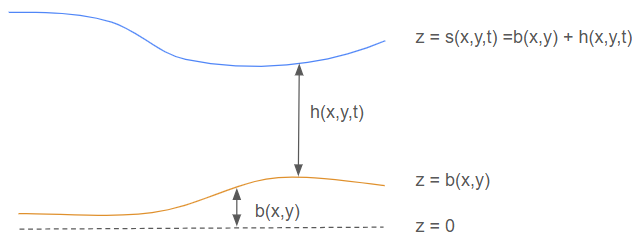
\includegraphics[width=0.5\textwidth]{figs/water-column-bc.png}
    \caption{Illustration of a water column with a free surface.}\label{fig:water_column_bc}
\end{figure}
We impose boundary conditions at the bottom and the free surface, adressing both kinematic and dynamical conditions.
Assume that a boundary is described by the function 
\begin{align*}
    \psi(x,y,z,t) = 0.
\end{align*}
For the free surface, this boundary is given by
\begin{align}\label{eq:psi_free_surface}
    \psi(x,y,z,t) \equiv z - s(x,y,t) = 0,
\end{align}
and for the bottom, it is described by
\begin{align}\label{eq:psi_bottom}
    \psi(x,y,z,t) \equiv z - b(x,y) = 0.
\end{align}
In the kinematic condition, we assume that fluid particles on the boundary remain on the boundary over time.
It is given by
\begin{align}\label{eq:kinematic_condition}
    \frac{\text{d} }{\text{d} t} \psi(x,y,z,t) = \psi_t + u \psi_x + v \psi_y + w \psi_z = 0.
\end{align}
Applying this to the free surface by substituting~\eqref{eq:psi_free_surface} into the kinematic condition~\eqref{eq:kinematic_condition} yields
\begin{align}\label{eq:kinematic_condition_free_surface}
    (s_t + u s_x + v s_y - w)|_{z=s} = 0.
\end{align}
Similarly, for the bottom, substitung~\eqref{eq:psi_bottom} into the kinematic condition~\eqref{eq:kinematic_condition} gives
\begin{align}\label{eq:kinematic_condition_bottom}
    (b_t + u b_x + v b_y - w)|_{z=b} = 0.
\end{align}
The dynamical condition is related to the pressure distribution at the free surface.
We assume that the pressure at the free surface is equal to the pressure in the air above the surface, that is, the atmospheric pressure.
Since absolute pressure levels are irrelevant (we are primarily concerned with pressure differences), we set the pressure at the free surface to zero.
This leads to the following expression for the pressure at the free surface:
\begin{align}\label{eq:pressure_free_surface}
    p(x,y,z,t)|_{z = s(x,y)} = p_{atm} = 0.
\end{align}
This condition, known as the dynamical condition, relates to the forces acting on the boundaries of the fluid.

\subsection{Assumptions}
To derive the SWE it is neccessary to make some assumptions. 
The shallow water equations are an approximation to the full free-surface problem and result from the assumption that the vertical compononent of the acceleration is negligible.
We begin by assuming that the vertical acceleration, represented by the total derivate of the vertical velocity component $w$ with respect to time, is negligible.
This assumption leads to the condition
\begin{align*}%\label{eq:assumption_dwdt}
    \frac{\text{d} w}{\text{d} t} = w_t + uw_x + vw_y + ww_z = 0.
\end{align*}
Here, $\frac{\partial w}{\partial t}$ is the partial derivative of $w$ with respect to $t$, while the total derivate $\frac{\text{d} w}{\text{d} t}$ accounts for both the direct change of $w$ with $t$ and the changes due to the movement of the fluid in the $x, y$ and $z$ directions.
Recall, that mathematically, the total derivative of $w$ wrt. $t$ is given by
\begin{align*}
    \frac{\text{d} w}{\text{d} t} &= \frac{\partial w}{\partial t} + \frac{\text{d} x}{\text{d} t} \frac{\partial w}{\partial x} + \frac{\text{d} y}{\text{d} t}  \frac{\partial w}{\partial y} + \frac{\text{d} z}{\text{d} t}  \frac{\partial w}{\partial z} \\
    &= w_t + u w_x + u w_y + w w_z .
\end{align*}
Applying $\text{d }w/\text{d }t = 0$ in the $z-$momentum conservation equation~\eqref{eq:momentum_conservation_z} simplifies it to
\begin{align*}
    p_z = -\rho g.
\end{align*}
This implies the pressure distribution follows
\begin{align}\label{eq:pressure_distribution}
    p = \int_z^s - \rho g \text{ d} z = \rho g (s - z),
\end{align}
where $s$ is the surface height.
Differentiating~\eqref{eq:pressure_distribution} with respect to $x$ and $y$ yields
\begin{align*}%\label{eq:pressure_distribution_x_y}
    p_x = \rho g s_x, \quad p_y = \rho g s_y.
\end{align*}
Substituting these expressions into the $x-$ and $y-$momentum conservation equations~\eqref{eq:momentum_conservation_x} and~\eqref{eq:momentum_conservation_y} leads to 
\begin{align}\label{eq:momentum_conservation_x_simplified}
    u_t + u u_x + v u_y + w u_z = -g s_x, 
\end{align}
and
\begin{align}\label{eq:momentum_conservation_y_simplified}
    v_t + u v_x + v v_y + w v_z = -g s_y.
\end{align}
These are the simplified momentum equations for the shallow water equations.
We realize that $p_x$ and $p_y$ are both independent of $z$, implying that $\text{d }u/ \text{d }t$ and $\text{d }v/ \text{d }t$ are also independent of $z$.
Hence $u_z = v_z = 0$, implying that~\eqref{eq:momentum_conservation_x_simplified} and~\eqref{eq:momentum_conservation_y_simplified} can be simplified to
\begin{align}\label{eq:momentum_conservation_x_final}
    u_t + u u_x + v u_y = -g s_x, 
\end{align}
and
\begin{align}\label{eq:momentum_conservation_y_final}
    v_t + u v_x + v v_y = -g s_y.
\end{align}


\subsection{Integration over depth}
The next step in deriving the SWE is to integrate the equations over the vertical direction.
We integrate the mass conservation equation~\eqref{eq:mass_conservation_incompressible} and the momentum conservation equations~\eqref{eq:momentum_conservation_x},~\eqref{eq:momentum_conservation_y} from the bottom, $z = b(x,y)$ to the free surface, $z = s(x,y,t)$.
Starting with the mass conservation equation~\eqref{eq:mass_conservation_incompressible}, we have
\begin{align*}
    \int_{b}^{s} u_x + v_y + w_z \text{ d} z = 0,
\end{align*}
implying that, using linearity of the integral:
\begin{align}\label{eq:mass_conservation_integrated}
    \int_{b}^{s} u_x \text{ d} z + \int_{b}^{s} v_y \text{ d} z  + w|_{z = s} - w|_{z = b} = 0.
\end{align}
We will use Leibniz's integral rule~\cite{Leibniz}, which is stated as follows:
\begin{align}\label{eq:leibniz_rule}
    \frac{\text{d}}{\text{d} x} \int_{a(x)}^{b(x)} f(x,t) \text{ d} t
    = \int_{a(x)}^{b(x)} \frac{\partial }{\partial x} f(x, t) \text{ d} t + f(x, b(x)) \frac{\text{d}}{\text{d} x} b(x) - f(x, a(x)) \frac{\text{d}}{\text{d} x} a(x),
\end{align}
to integrate the first two terms on the right hand side in~\eqref{eq:mass_conservation_integrated}, which yields
\begin{align*}
    \int_{b}^{s} u_x \text{d} z =  \frac{\text{d}}{\text{d} x}  \int_{b}^{s} u \text{ d} z  - u|_{z = s} \frac{\text{d} s}{\text{d} x} + u|_{z = b} \frac{\text{d} b}{\text{d} x}
\end{align*}
and 
\begin{align*}
    \int_{b}^{s} v_y \text{ d} z =  \frac{\text{d}}{\text{d} y}  \int_{b}^{s} v \text{ d} z  - v|_{z = s} \frac{\text{d} s}{\text{d} y} + u|_{z = b} \frac{\text{d} b}{\text{d} y}.
\end{align*}
Note that since a change in $x$ does not affect the $y$-component of the bottom or surface, we have that $\text{d} s/\text{d} x = s_x$ and $\text{d} b / \text{d} x = b_x$, and correspondingly for $s_y$ and $b_y$.
Likewise we can substitute $\frac{\text{d}}{\text{dx}}$ with $\frac{\partial}{\partial x}$ in the integrals, since the integrals are with respect to $z$.
Inserting these results in the above equations gives
\begin{align}
    \int_{b}^{s} u_x \text{ d} z =  \frac{\partial}{\partial x}  \int_{b}^{s} u \text{ d} z  - u|_{z = s} s_x + u|_{z = b} b_x
\end{align}
and 
\begin{align}
    \int_{b}^{s} v_y \text{ d} z = \frac{\partial}{\partial y}  \int_{b}^{s} v \text{ d} z  - v|_{z = s} s_y + u|_{z = b} b_y.
\end{align}
Inserting these results in~\eqref{eq:mass_conservation_integrated} gives
\begin{align}\label{eq:mass_conservation_integrated_final}
    \frac{\partial}{\partial x}  \int_{b}^{s} u \text{ d} z  - u|_{z = s} s_x + u|_{z = b} b_x
    + \frac{\partial}{\partial y}  \int_{b}^{s} v \text{ d} z  - v|_{z = s} s_y + u|_{z = b} b_y
    + w|_{z = s} - w|_{z = b} = 0.
\end{align}
From~\eqref{eq:kinematic_condition_bottom} we have
\begin{align}
    w|_{z = b} = (u b_x + v b_y)|_{z = b},
\end{align}
and from~\eqref{eq:kinematic_condition_free_surface} we have
\begin{align}
    w|_{z = s} = (s_t + u s_x + v s_y)|_{z = s}.
\end{align}
Realizing that $s = b + h$ and hence $s_t = h_t$, as the bottom is fixed.
Recall that $u$ and $v$ are independent of $z$, and the water depth is $h = s - b$, meaning we have
\begin{align*}
    \int_{b}^{s} u \text{ d} z = u(s - b) = hu, \quad \int_{b}^{s} v \text{ d} z = v(s - b) = hv.
\end{align*}
Putting it all together~\eqref{eq:mass_conservation_integrated_final} simplifies to
\begin{align}\label{eq:SWE_1}
    h_t + {(hu)}_x + {(hv)}_y = 0,
\end{align}
which is also the first equation in the SWE in conservative form.
When integrating the momentum equations~\eqref{eq:momentum_conservation_x_final} and~\eqref{eq:momentum_conservation_y_final} over the vertical direction, we see that since the equations are independent of $z$, the resulting equations are simply
\begin{align}
    h(u_t + uu_x + vu_y + g s_x) &= 0, \label{eq:x_momentum} \\
    h(v_t + uv_x + vv_y + g s_y) &= 0. \label{eq:y_momentum}
\end{align}
We multiply~\eqref{eq:SWE_1} with $u$ and $v$ respectively, and add the two equations to~\eqref{eq:x_momentum} and~\eqref{eq:y_momentum} correspondingly.
Recall that $s = h + b$. 
By using the product rule for differentiation and collecting terms, we obtain the momentum equations in conservative form:
\begin{align*}
    {(hu)}_t + {(hu^2 + \frac{1}{2}gh^2)}_x + {(huv)}_y = -gh b_x,
\end{align*}
and 
\begin{align*}
    {(hv)}_t + {(huv)}_x + {(hv^2 + \frac{1}{2}gh^2)}_y = -gh b_y.
\end{align*}



\subsection{The SWE in vector form for 1D and 2D}
The SWE, which consist of three partial differential equations, can be written in differential conservation law form as a vector equation
\begin{align}
    \mathbf{U}_t + \mathbf{F(U)}_x + \mathbf{G(U)}_y = \mathbf{S(U)},
\end{align}
where 
\begin{align*}
    \mathbf{U} = \begin{bmatrix}
        h \\
        hu \\
        hv
    \end{bmatrix},
    \quad 
    \mathbf{F(U)} = \begin{bmatrix}
        hu \\
        hu^2 + \frac{1}{2}gh^2 \\
        huv
    \end{bmatrix},
    \quad
    \mathbf{G(U)} = \begin{bmatrix}
        hv \\
        huv \\
        hv^2 + \frac{1}{2}gh^2
    \end{bmatrix}
    \quad \text{and} \quad
    \mathbf{S(U)} = \begin{bmatrix}
        s_1 \\
        s_2 \\
        s_3
    \end{bmatrix}.
\end{align*}
We call $\mathbf{U}$ the vector of conserved variables, $\mathbf{F(U)}$ and $\mathbf{G(U)}$ the flux vectors in the $x$ and $y$ direction, and $\mathbf{S(U)}$ the source term vector.

In this project, we will begin by considering the homogenneous one-dimensional case, where the flow is only in the $x$-direction:
\begin{align*}
    \mathbf{U}_t + {\mathbf{F(U)}}_x = 0,
\end{align*}
where 
\begin{align*}
    \mathbf{U} = \begin{bmatrix}
        h \\
        hu
    \end{bmatrix},
    \quad
    \text{and} \quad
    \mathbf{F(U)} = \begin{bmatrix}
        hu \\
        hu^2 + \frac{1}{2}gh^2
    \end{bmatrix}.
\end{align*}
%These equations are also known as the Saint Venant equations.




